\documentclass{article}
\usepackage{geometry}
\usepackage{graphicx}
\usepackage{amsmath}
\usepackage{xcolor}
\begin{document}
\setlength{\unitlength}{1cm}
\begin{picture}(20,15)
  \put(0,0){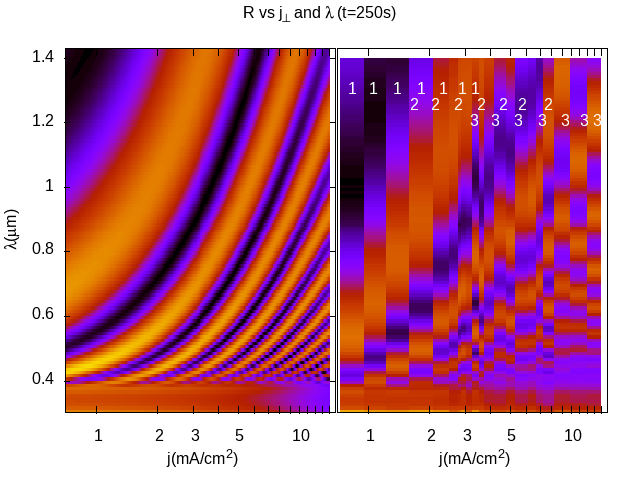
\includegraphics[width=\textwidth]{fig13}}
  \put(2.5,1){\color{white}
    \put(0,5){\scalebox{1.5}{Spectra calculated}}
    \put(0,4){\scalebox{1.5}{from fit.}}
  }
  \put(8.5,1){\color{white}
    \put(0,5){\scalebox{1.5}{Spectra measured at}}
    \put(0,4){\scalebox{1.5}{7 positions on each of}}
    \put(0,3){\scalebox{1.5}{3 samples with}}
    \put(0,2){\scalebox{1.5}{$I_1<I_2<I_3$}}
  }
\end{picture}
\end{document}